%
% teil3.tex -- Beispiel-File für Teil 3
%
% (c) 2020 Prof Dr Andreas Müller, Hochschule Rapperswil
%
\section{Beispiel einer Verfolgungskurve
\label{lambertw:section:teil4}}
\rhead{Beispiel einer Verfolgungskurve}
In diesem Abschnitt wird rechnerisch das Beispiel einer Verfolgungskurve mit der Verfolgungsstrategie 1 beschreiben. Dafür werden zuerst Bewegungsraum, Anfangspositionen und Bewegungsverhalten definiert, in einem nächsten Schritt soll eine Differentialgleichung dafür aufgestellt werden und anschliessend gelöst werden.

\subsection{Anfangsbedingungen definieren und einsetzen
	\label{lambertw:subsection:Anfangsbedingungen}}
Das zu verfolgende Ziel \(\vec{Z}\) bewegt sich entlang der \(y\)-Achse mit konstanter Geschwindigkeit \(v = 1\), beginnend beim Ursprung des Kartesischen Koordinatensystems. Der Verfolger \(\vec{V}\) startet auf einem beliebigen Punkt im ersten Quadranten und bewegt sich auch mit konstanter Geschwindigkeit \(|\dot{V}| = 1\) in Richtung Ziel. Diese Anfangspunkte oder Anfangsbedingungen können wie folgt formuliert werden:
\begin{equation}
	\vec{Z}
	=
	\left( \begin{array}{c} 0 \\ v \cdot t \end{array} \right)
	=
	\left( \begin{array}{c} 0 \\ t \end{array} \right)
	,\:
	\vec{V}
	=
	\left( \begin{array}{c} x \\ y \end{array} \right)
	\:\text{und}\:\:
	\bigl| \dot{V} \bigl|
	=
	1.
	\label{lambertw:Anfangsbed}
\end{equation}
Wir haben nun die Anfangsbedingungen definiert, jetzt fehlt nur noch eine DGL, welche die fortlaufende Änderung der Position und Bewegungsrichtung des Verfolgers beschreibt. 
Diese DGL haben wir bereits in Kapitel \ref{lambertw:subsection:Verfolger} definiert, und zwar Gleichung \eqref{lambertw:pursuerDGL}. Wenn man die Startpunkte einfügt ergibt sich folgender Ausdruck:
\begin{equation}
	\frac{\left( \begin{array}{c} 0-x \\ t-y \end{array} \right)}{\sqrt{x^2 + (t-y)^2}}
	\cdot
	\left(\begin{array}{c} \dot{x} \\ \dot{y} \end{array}\right)
	=
	1.
	\label{lambertw:eqMitAnfangsbed}
\end{equation}

\subsection{DGL vereinfachen
	\label{lambertw:subsection:DGLvereinfach}}
Nun haben wir eine Gleichung, es stellt sich aber die Frage ob es überhaupt eine geschlossene Lösung dafür gibt. Eine Funktion welche die Beziehung \(y(x)\) beschreibt oder sogar \(x(t)\) und \(y(t)\) liefert. Zum jetzigen Zeitpunkt mag es nicht trivial scheinen, aber mit den gewählten Anfangsbedingungen \eqref{lambertw:Anfangsbed} ist es möglich eine geschlossene Lösung für die Gleichung \eqref{lambertw:eqMitAnfangsbed} zu finden.
Auf dem Weg dahin muss die definierte DGL zuerst wesentlich vereinfacht werden, sei es mittels algebraische Umformungen oder mit den Tools aus der Analysis. Also legen wir los! 

Zuerst müssen wir den Bruch in \eqref{lambertw:eqMitAnfangsbed} los werden, der sieht so nicht handlich aus. Dafür multiplizieren wir beidseitig mit dem Nenner:
\begin{equation}
	\left( \begin{array}{c} 0-x \\ t-y \end{array} \right)
	\cdot
	\left(\begin{array}{c} \dot{x} \\ \dot{y} \end{array}\right)
	= \sqrt{x^2 + (t-y)^2}.
	\label{lambertw:eqOhneBruch}
\end{equation}
In einem weiteren Schritt, lösen wir das Skalarprodukt auf und erhalten folgende Gleichung \eqref{lambertw:eqOhneSkalarprod} ohne vektorielle Grössen:
\begin{equation}
		-x \cdot \dot{x} + (t-y) \cdot \dot{y}
		= \sqrt{x^2 + (t-y)^2}.
		\label{lambertw:eqOhneSkalarprod}
\end{equation}
Im letzten Schritt, fällt die Nützlichkeit des Skalarproduktes in der Verfolgungsgleichung \eqref{lambertw:pursuerDGL} markant auf. Meiner Meinung ziemlich elegant und nicht selbstverständlich in der Lage zu sein, das Problem auf eine einzige Gleichung reduzieren zu können.

Die nächsten Schritte sind sehr algebralastig und würden das lesen dieses Papers einfach nur mühsam machen, also werde ich diese auslassen. Hingegen werden ich die algebraische Hauptschritte erwähnen, die notwendig wären falls man es trotzdem selber ausprobieren möchte:
\begin{itemize}
	\item
	Quadrieren und erweitern.
	\item
	Gruppieren.
	\item
	Substitution von einzelnen Thermen mittels der Beziehung \(\dot{x}^2 + \dot{y}^2 = 1\).
	\item
	Und das erkennen des Musters einer Binomischen Formel.
\end{itemize} 
Das Resultat aller dieser Vereinfachungen führen zu folgender Gleichung \eqref{lambertw:eqAlgVerinfacht}, die viel handhabbarer ist als zuvor:
\begin{equation}
	(x \dot{y} + (t-y) \dot{x})^2
	= 0.
	\label{lambertw:eqAlgVerinfacht}
\end{equation}
Da der linke Term gleich Null ist, muss auch der Inhalt des Quadrates gleich Null sein, somit folgt eine weitere Vereinfachung, welche zu einer im Vergleich zu \eqref{lambertw:eqOhneSkalarprod} wesentlich einfachere DGL führt:
\begin{equation}
	x \dot{y} + (t-y) \dot{x}
	= 0.
	\label{lambertw:eqGanzVerinfacht}
\end{equation}
Kompakt, ohne Wurzelterme und Quadrate, nur elementare Operationen und Ableitungen. Nun stellt sich die Frage wie es weiter gehen soll, bei der Gleichung \eqref{lambertw:eqGanzVerinfacht} scheinen keine weiteren Vereinfachungen möglich zu sein. Wir brauchen einen neuen Ansatz um unser Ziel einer möglichen Lösung zu verfolgen.

\subsection{Zeitabhängigkeit loswerden
	\label{lambertw:subsection:ZeitabhLoswerden}}
Der nächste logischer Schritt schient irgendwie die Zeitabhängigkeit in der Gleichung \eqref{lambertw:eqGanzVerinfacht} loszuwerden, aber wieso? Nun, wie am Anfang von Abschnitt \ref{lambertw:subsection:DGLvereinfach} beschrieben, suchen wir eine Lösung der Art \(y(x)\), dies ist natürlich erst möglich wenn wir die Abhängigkeit nach \(t\) eliminieren können.

Der erste Schritt auf dem Weg dahin, ist es die zeitlichen Ableitung los zu werden, dafür wird \eqref{lambertw:eqGanzVerinfacht} beidseitig mit \(\dot{x}\) dividiert, was erlaubt ist, weil diese Änderung ungleich Null ist:
\begin{equation}
	x \frac{\dot{y}}{\dot{x}} + (t-y) \frac{\dot{x}}{\dot{x}}
	= 0.
	\label{lambertw:eqVorKeineZeitAbleit}
\end{equation}
Der Grund dafür ist, dass
\begin{equation}
	\frac{\displaystyle\dot{y}}{\displaystyle\dot{x}} 
	= \frac{\displaystyle\frac{dy}{dt}}{\displaystyle\frac{dx}{dt}}  
	= \frac{dy}{dx}
	= y^{\prime},
	\label{lambertw:eqQuotZeitAbleit}
\end{equation}
und somit kann der Quotient dieser zeitlichen Ableitungen in eine Ableitung nach \(x\) umgewandelt werden.
Nach dem diese Eigenschaft \eqref{lambertw:eqQuotZeitAbleit} in \eqref{lambertw:eqVorKeineZeitAbleit} eingesetzt wird und vereinfacht wurde, entsteht folgende neue Gleichung:
\begin{equation}
	x y^{\prime} + t - y
	= 0.
	\label{lambertw:DGLmitT}
\end{equation}
Hier wäre es natürlich passend wenn man die Abhängigkeit nach \(t\) komplett wegbringen könnte. Um dies zu erreichen muss man auf die Definition der Bogenlänge aus der Analysis zurückgreifen, wobei die Strecke \(s\) folgendem entspricht:
\begin{equation}
	s
	= 
	v \cdot t
	=
	1 \cdot t
	=
	t
	=
	\int_{\displaystyle x_0}^{\displaystyle x_{\text{end}}}\sqrt{1+y^{\prime\, 2}} \: dx.
	\label{lambertw:eqZuBogenlaenge}
\end{equation}
Nicht gerade auffällig ist die Richtung in welche hier integriert wird. Wenn der Verfolger sich wie vorgesehen am Anfang im ersten Quadranten befindet, dann muss sich dieser nach links bewegen, was nicht der üblichen Integrationsrichtung entspricht. Um eine Integration wie üblich von links nach rechts ausführen zu können, müssen die Integrationsgenerzen vertauscht werden, was in einem Vorzeichenwechsel resultiert. Wenn man nun \eqref{lambertw:eqZuBogenlaenge} in die DGL \eqref{lambertw:DGLmitT} einfügt, dann ergibt sich folgender Ausdruck:
\begin{equation}
	x y^{\prime} - \int\sqrt{1+y^{\prime\, 2}} \: dx - y
	= 0.
	\label{lambertw:DGLohneT}
\end{equation}
Um das Integral los zu werden, leitet man den vorherigen Ausdruck \eqref{lambertw:DGLohneT} nach \(x\) ab und erhaltet folgende DGL \eqref{lambertw:DGLohneInt}:
\begin{align}
	y^{\prime}+ xy^{\prime\prime} - \sqrt{1+y^{\prime\, 2}} - y^{\prime}
	&= 0, \\
	xy^{\prime\prime} - \sqrt{1+y^{\prime\, 2}}
	&= 0.
	\label{lambertw:DGLohneInt}
\end{align}
Nun sind wir unserem Ziel einen weiteren Schritt näher. Die Gleichung \eqref{lambertw:DGLohneInt} mag auf den ersten Blick nicht gerade einfach sein, aber im Nächsten Abschnitt werden wir sehen, dass sie relativ einfach zu lösen ist.

\subsection{DGL lösen
	\label{lambertw:subsection:DGLloes}}
Die Gleichung \eqref{lambertw:DGLohneInt} ist eine DGL zweiter Ordnung und kann 
mittels der Substitution \(y^{\prime} = u\) in eine DGL erster Ordnung umgewandelt werden:
\begin{equation}
	xu^{\prime} - \sqrt{1+u^2}
	= 0.
	\label{lambertw:DGLmitU}
\end{equation}
Diese \eqref{lambertw:DGLmitU} zu lösen ist ziemlich einfach da sie separierbar ist, aus diesem Grund werde ich direkt zur Lösung \eqref{lambertw:loesDGLmitU} übergehen:
\begin{align}
	\operatorname{arsinh}(u)
	&=
	\operatorname{ln}(x) + C, \\
	u
	&=
	\operatorname{sinh}(\operatorname{ln}(x) + C).
	\label{lambertw:loesDGLmitU}
\end{align}
Indem man die Substitution rückgängig macht, erhält man eine weitere DGL erster Ordnung die bereits separiert ist und erhält folgende Gleichung:
\begin{equation}
	y^{\prime}
	=
	\operatorname{sinh}(\operatorname{ln}(x) + C).
	\label{lambertw:loesDGLmitY}
\end{equation}
Diese \eqref{lambertw:loesDGLmitY} kann mit den selben Methoden gelöst werden wie \eqref{lambertw:DGLmitU}, diesmal aber in Kombination mit der exponentiellen Definition der \(\operatorname{sinh}\)-Funktion:
\begin{equation}
	y
	=
	C_1 + C_2 x^2 - \frac{\operatorname{ln}(x)}{8 \cdot C_2}.
\end{equation}
Nun haben wir eine Lösung, aber wie es immer mit Lösungen ist, stellt sich die Frage ob sie überhaupt plausibel ist. Dieser Frage werden wir in nächsten Abschnitt \ref{lambertw:subsection:LoesAnalys} nachgehen.

\subsection{Lösung analysieren
	\label{lambertw:subsection:LoesAnalys}}

\begin{figure}
	\centering
	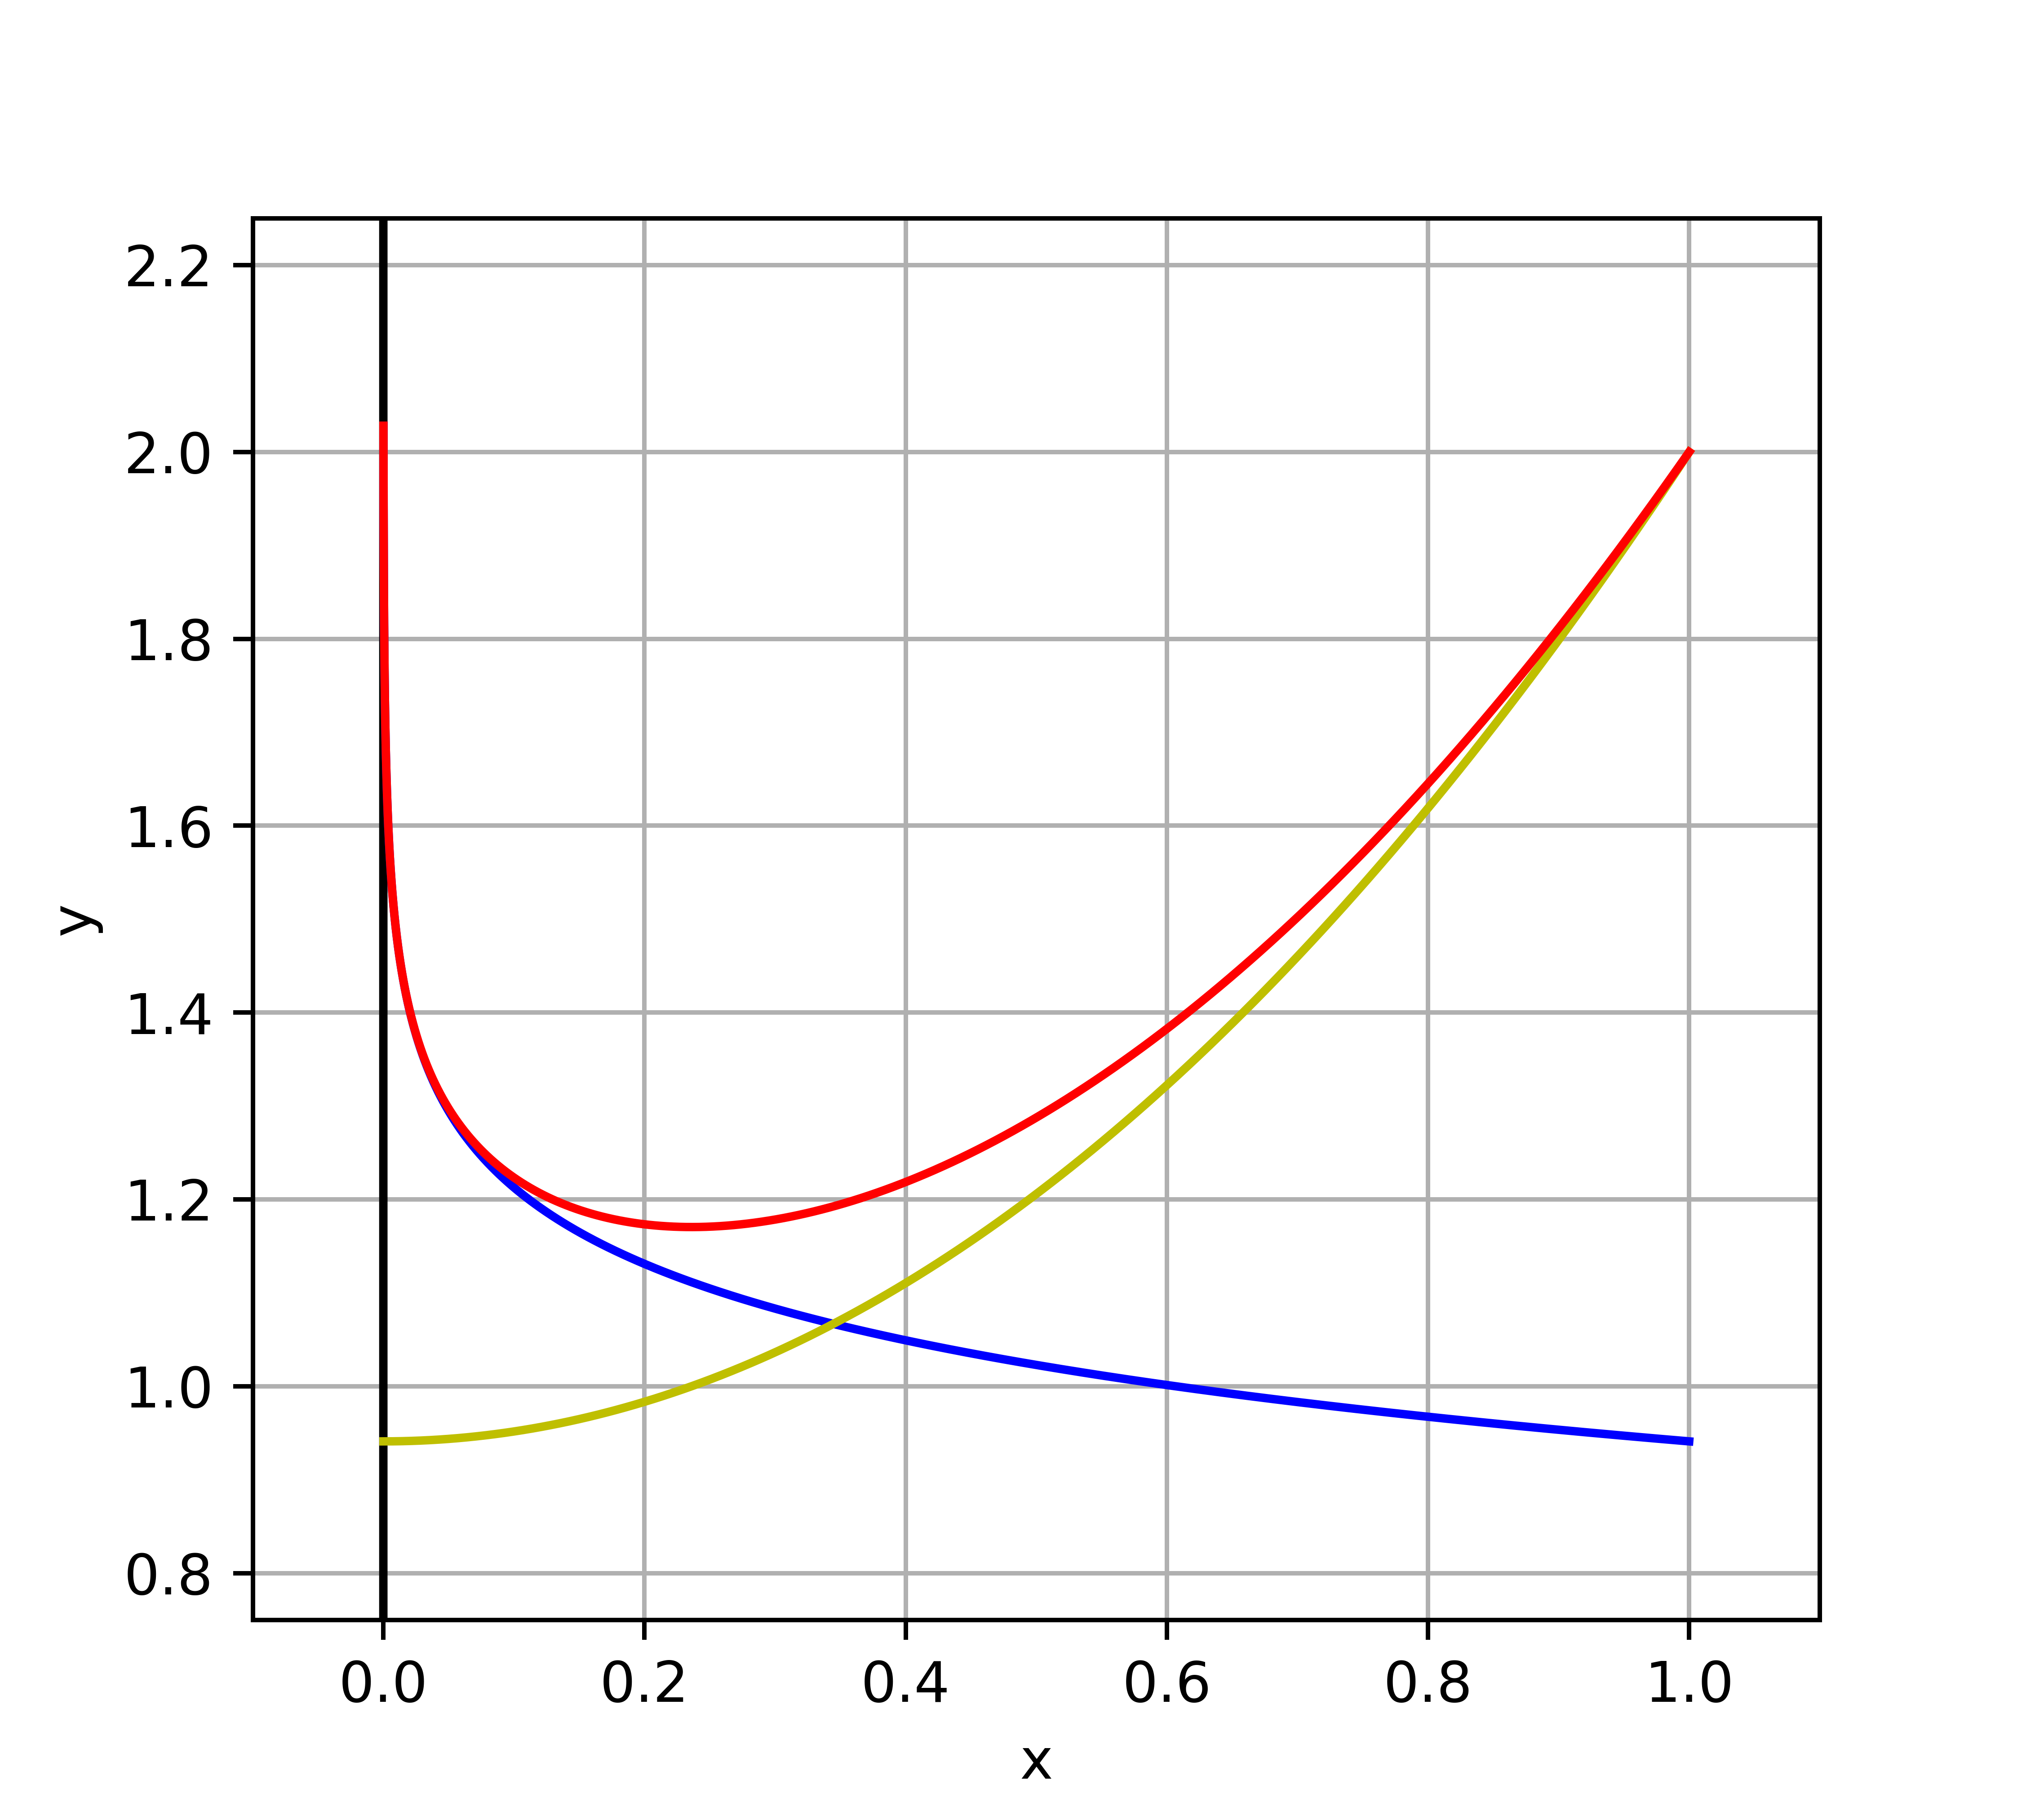
\includegraphics{papers/lambertw/Bilder/VerfolgungskurveBsp.png}
	\caption[Graph der Verfolgungskurve]{Graph der Verfolgungskurve wobei, ({\color{red}rot}) die Funktion \ensuremath{y(x)} ist, ({\color{darkgreen}grün}) der quadratische Teil und ({\color{blue}blau}) dem \ensuremath{ln(x)}-Teil entspricht.
	\label{lambertw:BildFunkLoes}
	}
\end{figure}

Das Resultat, wie ersichtlich, ist folgende Funktion \eqref{lambertw:funkLoes} welche mittels Anfangsbedingungen parametrisiert werden kann: 
\begin{equation}
	{\color{red}{y(x)}}
	=
	C_1 + C_2 {\color{darkgreen}{x^2}} {\color{blue}{-}} \frac{\color{blue}{\operatorname{ln}(x)}}{8 \cdot C_2}.
	\label{lambertw:funkLoes}
\end{equation}
Für die Koeffizienten \(C_1\) und \(C_2\) ergibt sich ein Anfangswertproblem, welches für deren Bestimmung gelöst werden muss. Zuerst soll aber eine qualitative Intuition, oder Idee für das Aussehen der Funktion \(y(x)\) geschaffen werden:
\begin{itemize}
	\item
	Für grosse \(x\)-Werte, welche in der Regel in der Nähe von \(x_0\) sein sollten, ist der quadratisch Term in der Funktion \eqref{lambertw:funkLoes} dominant. 
	\item
	Für immer kleiner werdende \(x\) geht der Verfolger in Richtung \(y\)-Achse, wobei seine Steigung stetig sinkt, was Sinn macht wenn der Verfolgte entlang der \(y\)-Achse steigt. Irgendwann werden Verfolger und Ziel auf gleicher Höhe sein.
	\item
	Für \(x\)-Werte in der Nähe von \(0\) ist das asymptotische Verhalten des Logarithmus dominant, dies macht auch Sinn da sich der Verfolgte auf der \(y\)-Achse bewegt und der Verfolger im nachgeht.
	\item
	Aufgrund des Monotoniewechsels in der Kurve \eqref{lambertw:funkLoes} muss diese auch ein Minimum aufweisen. Es stellt sich nun die Frage: Wo befindet sich dieser Punkt? 
	
	Eine Abschätzung darüber kann getroffen werden und zwar, dass dieser dann entsteht, wenn \(A\) und \(P\) die gleiche \(y\)-Koordinaten besitzen. In diesem Moment ändert die Richtung der \(y\)-Komponente der Geschwindigkeit des Verfolgers, somit auch sein Vorzeichen und dadurch entsteht auch das Minimum.
\end{itemize}
Alle diese Eigenschafte stimmen mit dem überein, was man von einer Kurve dieser Art erwarten würde, welche durch die Grafik \ref{lambertw:BildFunkLoes} repräsentiert wurde. Nun stellt sich die Frage wie die Kurve wirklich aussieht. Dies wird im folgenden Abschnitt \ref{lambertw:subsection:AllgLoes} behandelt.

\subsection{Anfangswertproblem 
	\label{lambertw:subsection:AllgLoes}}
Wie üblich bei der Suche nach einer exakten Lösung, kommt ein Anfangswertproblem vor. Um dieses zu lösen, müssen wir zuerst die Anfangswerte definieren. Da wir das Problem allgemein lösen wollen, ergeben sich folgende zwei Anfangswerte:
\begin{equation}
	y(x)\big \vert_{t=0}
	=
	y(x_0)
	= 
	y_0
	\label{lambertw:eq1Anfangswert}
\end{equation}
und
\begin{equation}
	\frac{dy}{dx}\bigg \vert_{t=0}
	=
	y^{\prime}(x_0)
	=
	\frac{y_0}{x_0}.
	\label{lambertw:eq2Anfangswert}
\end{equation}
Der zweite Anfangswert \eqref{lambertw:eq2Anfangswert} mag nicht grade offensichtlich sein. Die Erklärung dafür ist aber simpel: Der Verfolger wird sich zum Zeitpunkt \(t=0\) in Richtung Koordinatenursprung bewegen wollen, wo sich das Ziel befindet. Somit entsteht das Steigungsdreieck mit \(\Delta x = x_0\) und \(\Delta y = y_0\).

Das Lösen des Anfangswertproblems ist ein Problem aus der Algebra, auf welches ich nicht unbedingt eingehen möchte. Zur Vollständigkeit und Nachvollziehbarkeit, werde ich aber das Gleichungssystem \eqref{lambertw:eqGleichungssystem} präsentieren, welches notwendig ist um das Anfangswertproblem zu lösen, sowie auch die allgemeine Lösung \eqref{lambertw:eqAllgLoes} die sich nach dem einsetzen der Koeffizienten \(C_1\) und \(C_2\) in die Funktion \eqref{lambertw:funkLoes} ergibt.

\begin{itemize}
	\item
	Gleichungssystem:
	\begin{subequations}
		\begin{align}
			y_0
			&=
			C_1 + C_2 x^2_0 - \frac{\operatorname{ln}(x_0)}{8 \cdot C_2}, \\
			\frac{y_0}{x_0}
			&=
			2 \cdot  C_2 x_0 - \frac{1}{8 \cdot C_2 \cdot x_0}.
		\end{align}
		\label{lambertw:eqGleichungssystem}
	\end{subequations}
	\item
	Die allgemeine Funktion:
	\begin{equation}
		y(x)
		=
		\frac{1}{4}\left(\left(y_0+r_0\right)\eta+\left(r_0-y_0\right)\operatorname{ln}\left(\eta\right)-r_0+3y_0\right)
		\label{lambertw:eqAllgLoes}
	\end{equation}
	Damit die Funkion \eqref{lambertw:eqAllgLoes} trotzdem noch übersichtlich bleibt, wurden \(\eta\) und \(r_0\) wie folgt definiert:
	\begin{equation}
		\eta
		=
		\left(\frac{x}{x_0}\right)^2
		\:\:\text{und}\:\:
		r_0
		=
		\sqrt{x_0^2+y_0^2}.
	\end{equation}
\end{itemize}
Diese neue allgemein Funktion \eqref{lambertw:eqAllgLoes} weist immer noch die selbe Struktur wie die vorherig hergeleitete Funktion \eqref{lambertw:funkLoes} auf, einerseits einen quadratischen Teil der in \(\eta\) enthalten ist, anderseits den \(\operatorname{ln}\)-Teil. Aus dieser Ähnlichkeit kann geschlossen werden, dass sich \eqref{lambertw:eqAllgLoes} auf eine ähnliche Art verhalten wird.

Nun sind wir soweit, dass wir eine \(y(x)\)-Beziehung für beliebige Anfangswerte darstellen können, unser erstes Ziel wurde erreicht. Ist das alles? Nein, wir können einen Schritt weiter gehen und uns Fragen: Ist es analytisch möglich herauszufinden, wo sich Verfolger und Ziel zu jedem Zeitpunkt befinden? Dieser Frage werden wir im nächsten Abschnitt nachgehen.

\subsection{Funktion nach der Zeit 
	\label{lambertw:subsection:FunkNachT}}
Lieber Leser sei mir nicht böse, aber in diesem Abschnitt werde ich ein wenig mehr bei den algebraischen Umformungen ins Detail gehen. Dies hat auch einen bestimmten Grund, ich möchte den Einsatz einer speziellen Funktion aufzeigen, sowie auch wann und wieso diese vorkommt. Welche spezielle Funktion? Fragst du dich wahrscheinlich in diesem Moment. Nun, um diese Frage zu kurz zu beantworten, es ist "YouTube's favorite special function" laut dem Mathematiker Michael Penn, die Lambert-W-Funktion \(W(x)\) welche übrigens im Kapitel \ref{buch:section:lambertw} bereits beschrieben wurde.

Also fangen wir an. Der erste Schritt ist es herauszufinden, wie die Zeitabhängigkeit wieder hinein gebracht werden kann. Dafür greifen wir auf die letzte Gleichung zu, in welcher \(t\) noch enthalten war, und zwar DGL \eqref{lambertw:DGLmitT}, welche zur Übersichtlichkeit hier nochmals aufgeführt wird:
\begin{equation}
	x y^{\prime} + t - y
	= 0.
	\label{lambertw:eqDGLmitTnochmals}
\end{equation}
Wie in \eqref{lambertw:eqDGLmitTnochmals} zu sehen ist, werden \(y\) und deren Ableitung \(y^{\prime}\) benötigt, diese sind:
\begin{subequations}
	\begin{align}
		y
		&=
		\frac{1}{4}\left(\left(y_0+r_0\right)\eta+\left(r_0-y_0\right)\operatorname{ln}\left(\eta\right)-r_0+3y_0\right), \\
		\label{lambertw:eqFunkUndAbleit1}
		y^\prime
		&=
		\frac{1}{2}\left(\left(y_0+r_0\right)\frac{x}{x_0^2}+\left(r_0-y_0\right)\frac{1}{x}\right).
	\end{align}
	\label{lambertw:eqFunkUndAbleit}
\end{subequations}
Wenn man diese Gleichungen \ref{lambertw:eqFunkUndAbleit} in die DGL \label{lambertw:eqDGLmitTnochmals} einfügt, vereinfacht und nach \(t\) auflöst, dann ergibt sich folgenden Ausdruck:
\begin{equation}
	-4t
	=
	\left(y_0+r_0\right)\left(\eta-1\right)+\left(r_0-y_0\right)\operatorname{ln}\left(\eta\right).
	\label{lambertw:eqFunkUndAbleitEingefuegt}
\end{equation}
In einem nächsten Schritt wird alles mit \(x\) auf die eine Seite gebracht, der Rest auf die andere Seite und anschliessend beidseitig exponentiert, was wie folgt aussieht:
\begin{align}
	-4t+\left(y_0+r_0\right)
	&=
	\left(y_0+r_0\right)\eta+\left(r_0-y_0\right)\operatorname{ln}\left(\eta\right), \\
	e^{\displaystyle -4t+\left(y_0+r_0\right)}
	&=
	e^{\displaystyle \left(y_0+r_0\right)\eta}\cdot\eta^{\displaystyle \left(r_0-y_0\right)}.
	\label{lambertw:eqMitExp}
\end{align}
Auf dem rechten Term von \eqref{lambertw:eqMitExp} beginnen wir langsam eine ähnliche Struktur wie \(\eta e^\eta\) zu erkennen, dies schreit nach der Struktur die benötigt wird um \(\eta\) mittels der Lambert-W-Funktion \(W(x)\) zu erhalten. Dies macht durchaus Sinn, wenn wir die Funktion \(x(t)\) finden wollen und \(W(x)\) die Umkehrfunktion von \(x e^x\) ist. 

Die erste Sache die uns in \eqref{lambertw:eqMitExp} stört ist, dass \(\eta\) als Potenz da steht. Dieses Problem können wir loswerden, indem wir beidseitig mit \(\:\displaystyle \frac{1}{r_0-y_0}\:\) potenzieren:
\begin{equation}
	e^{\displaystyle \frac{-4t}{r_0-y_0}+\frac{y_0+r_0}{r_0-y_0}}
	=
	\eta\cdot e^{\displaystyle \frac{y_0+r_0}{r_0-y_0}\eta} .
	\label{lambertw:eqOhnePotenz}
\end{equation}
Das nächste Problem auf welches wir in \eqref{lambertw:eqOhnePotenz} treffen ist, dass \(\eta\) nicht alleine im Exponent steht. Dies kann elegant mit folgender Substitution gelöst werden:
\begin{equation}
	\chi
	=
	\frac{y_0+r_0}{r_0-y_0}.
	\label{lambertw:eqChiSubst}
\end{equation}
Es gäbe natürlich andere Substitutionen wie z.B. 
\[\displaystyle \chi=\frac{y_0+r_0}{r_0-y_0}\cdot\eta,\] 
die auf das selbe Ergebnis führen würden, aber \eqref{lambertw:eqChiSubst} liefert in einem Schritt die kompakteste Lösung. Also fahren wir mit der  Substitution \eqref{lambertw:eqChiSubst} weiter, setzen diese in die Gleichung \eqref{lambertw:eqOhnePotenz} ein und multiplizieren beidseitig mit \(\chi\). Daraus erhalten wir folgende Gleichung:
\begin{equation}
	\chi\cdot e^{\displaystyle \chi-\frac{4t}{r_0-y_0}}
	=
	\chi\eta\cdot e^{\displaystyle \chi\eta}.
	\label{lambertw:eqNachSubst}
\end{equation}
Schön oder? Nun sind wir endlich soweit, dass wir die angedeutete Lambert-W-Funktion \(W(x)\)einsetzen können. Wenn wir beidseitig \(W(x)\) anwenden, dann erhalten wir folgenden Ausdruck:
\begin{equation}
	W\left(\chi\cdot e^{\displaystyle \chi-\frac{4t}{r_0-y_0}}\right)
	=
	\chi\eta.
\end{equation}
Nach dem Auflösen nach \(x\) welches in \(\eta\) enthalten ist, erhalten wir die gesuchte \(x(t)\)-Funktion \eqref{lambertw:eqFunkXNachT}. Dieses \(x(t)\) in Kombination mit \eqref{lambertw:eqFunkUndAbleit1} liefert die Position des Verfolgers zu jedem Zeitpunkt. Das Gleichungspaar \eqref{lambertw:eqFunktionenNachT}, besteht aus folgenden Gleichungen:
\begin{subequations}
	\begin{align}
		\label{lambertw:eqFunkXNachT}
		x(t)
		&=
		x_0\cdot\sqrt{\frac{W\left(\chi\cdot e^{\displaystyle \chi-\frac{4t}{r_0-y_0}}\right)}{\chi}}, \\
		\label{lambertw:eqFunkYNachT}
		y(x(t))
		=
		y(t)
		&=
		\frac{1}{4}\left(\left(y_0+r_0\right)\left(\frac{x(t)}{x_0}\right)^2+\left(r_0-y_0\right)\operatorname{ln}\left(\left(\frac{x(t)}{x_0}\right)^2\right)-r_0+3y_0\right).
	\end{align}
	\label{lambertw:eqFunktionenNachT}
\end{subequations}
Nun haben wir unser letztes Ziel erreicht und sind in der Lage eine Verfolgung rechnerisch sowie graphisch zu repräsentieren.
 
Wir sind aber noch nicht ganz fertig, ich muss gestehen, dass ich in diesem Abschnitt einen wichtigen Teil verschwiegen habe. Und zwar wieso, dass ich schon bei der Gleichung \eqref{lambertw:eqFunkUndAbleitEingefuegt} wusste, dass man nach einigen Umformungen die Lambert-W-Funktion eingesetzt werden kann.
Der Grund dafür ist die Struktur
\begin{equation}
	y
	=
	p(x) +\operatorname{ln}(x),
	\label{lambertw:eqEinsatzLambW}
\end{equation}
bei welcher \(p(x)\) eine beliebige Potenz von \(x\) darstellt. 

Jedes mal wenn \(x\) gesucht ist und in einer Struktur der Art \eqref{lambertw:eqEinsatzLambW} vorkommt, dann kann mit ein paar Umformungen die Struktur \(f(x)e^{f(x)}\) erzielt werden. Wie bereits in diesem Abschnitt \ref{lambertw:subsection:FunkNachT} gezeigt wurde, kann \(x\) nun mittels der \(W(x)\)-Funktion aufgelöst werden. Erstaunlicherweise ist \eqref{lambertw:eqEinsatzLambW} eine Struktur die oftmals vorkommt, was die Lambert-W-Funktion so wichtig macht.